\chapter{Xây dựng và thiết kế giải pháp co dãn tài nguyên đa cấp độ chủ động cho ứng dụng SmartHome trong môi trường điện toán đám mây}

\section{Mô tả giải pháp}

\subsection{Mô tả yêu cầu hệ thống}

Để hỗ trợ việc hiện thực hóa các mục tiêu nghiên cứu, cần có một hệ thống được thiết kế và triển khai nhằm kiểm chứng tính khả thi của các đề xuất kỹ thuật. Phần này sẽ trình bày chi tiết kiến trúc tổng thể, các thành phần chức năng chính, cũng như mối liên kết giữa chúng. Việc mô tả rõ ràng hệ thống không chỉ giúp minh bạch hóa quá trình phát triển mà còn tạo tiền đề cho việc triển khai, đánh giá hiệu năng và khả năng mở rộng trong các phần sau.

\begin{figure}[htbp]
    \centering
    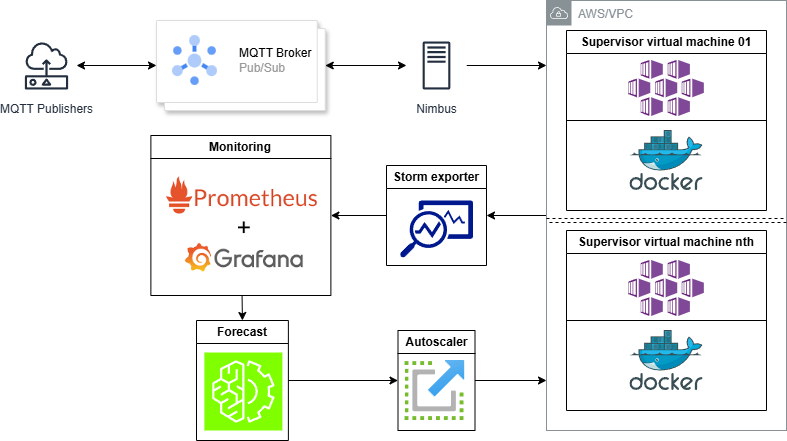
\includegraphics[width=\textwidth]{deployment-architect.drawio.png}
    \caption{Sơ đồ kiến trúc của hệ thống dự báo và co/dãn tài nguyên trên môi trường điện toán đám mây}
\end{figure}

Các thành phần của hệ thống:

\begin{itemize}
    \item \acrshort{mqtt} Publisher và Broker có vai trò gửi và chuyển các gói tin (dữ liệu nhà thông minh) đến các subscriber.
    \item Cụm Apache Storm gồm:
          \begin{itemize}
              \item Nimbus và Zookeeper điều phối và chỉ đạo các Supervisor.
              \item Supervisor chạy trong Docker container tại các máy ảo trên nền tảng cloud xử lý dữ liệu.
          \end{itemize}
    \item Storm exporter chịu trách nhiệm thu thập dữ liệu topology và các chỉ số của Docker.
    \item Prometheus thu thập dữ liệu chỉ số từ Storm exporter, Grafana có nhiệm vụ trực quan hóa các chỉ số này.
    \item Storm Forecast lấy các chỉ số từ Prometheus để dự đoán tài nguyên co/dãn.
    \item Storm autoscaler co/dãn tài nguyên supervisor.
\end{itemize}

Luồng dữ liệu sẽ thực hiện tuần tự như sau:

\begin{enumerate}
    \item Dữ liệu từ các thiết bị trong nhà thông minh được thu thập bởi \acrshort{mqtt} publisher sau đó được gửi đến \acrshort{mqtt} broker. \acrshort{mqtt} broker nhận dữ liệu và phân phối chúng đến các subscriber.
    \item Cụm Storm có các spout đóng vai trò subscriber nhận dữ liệu này và tiến hành xử lý dữ liệu. Do lượng dữ liệu trong hệ thống nhà thông minh không đồng đều tại các thời điểm khác nhau, tài nguyên hệ thống cần để đảm bảo xử lý dữ liệu kịp thời đáp ứng nhu cầu tải công việc cũng sẽ thay đổi.
    \item Storm exporter sẽ định kỳ thu thập các chỉ số từ các Supervisor thông qua Storm UI REST \gls{api} và Docker \gls{api}.
    \item Prometheus sẽ theo định kỳ thu thập các chỉ số từ Storm exporter để lưu trữ và phục vụ truy vấn.
    \item Grafana sẽ lấy dữ liệu từ nguồn Prometheus để trực quan hóa các chỉ số, hỗ trợ công việc vận hành, phân tích dữ liệu trực quan sau này và cung cấp cái nhìn tổng quát về hệ thống co/dãn.
    \item Storm Forecast thu thập các chỉ số từ Prometheus thông qua PromQL và số lượng máy ảo hiện tại từ Storm Autoscaler để tiến hành dự đoán tài nguyên co/dãn Supervisor.
    \item Storm autoscaler tiến hành co/dãn tài nguyên Supervisor dựa trên chỉ thị của Storm Forecast, sau đó autoscaler chờ 10 giây trước khi yêu cầu nimbus thực hiện lệnh tái phân phối (rebalance) các tiến trình công việc.
    \item Storm Forecast chờ 30 giây đến lần thực hiện hành động tiếp theo, tiến hành đo trạng thái môi trường lúc này làm đầu vào cho hàm đánh giá phần thưởng của cặp trạng thái môi trường với hành động trước đó.
\end{enumerate}

\subsubsection{Phương án triển khai}

Trong quá trình thiết kế hệ thống tự động co/dãn tài nguyên dựa trên học tăng cường, hai hướng triển khai thuật toán Q-learning thường được cân nhắc: (1) huấn luyện trực tiếp trong môi trường (online learning) và (2) chia tách thành hai giai đoạn huấn luyện – đánh giá (offline learning). Phương pháp học trực tiếp cho phép agent liên tục cập nhật chính sách dựa trên tương tác thực tế, từ đó thích nghi tốt với những thay đổi động của môi trường. Tuy nhiên, thời gian để học được một chính sách tốt có thể mất nhiều thời gian, nhất là với môi trường lớn/phức tạp như bài toán co/dãn tài nguyên cho ứng dụng nhà thông minh SmartHome.

Ngược lại, offline learning sử dụng dữ liệu lịch sử hoặc mô phỏng để huấn luyện trước một chính sách ban đầu, từ đó đảm bảo an toàn và kiểm soát tốt hơn quá trình học. Tuy nhiên, chính sách học được có thể thiếu tính linh hoạt trong các kịch bản chưa từng xuất hiện trong tập dữ liệu. Đặc biệt trong bài toán mà đề án này nghiên cứu hoạt động trên môi trường điện toán đám mây, có rất nhiều yếu tố ngoại cảnh sẽ ảnh hưởng đến hệ thống.

Vì vậy, để cân bằng giữa độ an toàn và khả năng thích ứng, đồ án sử dụng phương án kết hợp (hybrid): trước hết huấn luyện offline từ hệ thống mô phỏng, sau đó fine-tune chính sách thông qua học online trong môi trường điện toán đám mây. Cách tiếp cận này tận dụng ưu điểm của cả hai phương pháp, giúp hệ thống đạt hiệu quả co/dãn cao mà vẫn đảm bảo tính ổn định trong vận hành thực tế.

\paragraph{Yêu cầu của hệ thống}

Trên cơ sở kết quả phân tích bài toán và xác định phạm vi của đề tài đã được trình bày, sau đây sẽ là các đặc tả yêu cầu cụ thể mà hệ thống cần phải đáp ứng.

\begin{itemize}
    \item Cân bằng giữa việc mở rộng và thu hẹp: Đảm bảo không mở rộng quá mức khi hệ thống có chịu được tải, do môi trường triển khai trên hệ thống điện đoán đám mây, bất kỳ tài nguyên không hợp lý nào đều sẽ gây ra lãng phí. Không thu hẹp quá nhiều khiến hệ thống thiếu tài nguyên xử lý, gây ảnh hưởng nghiêm trọng đến trải nghiệm người dùng.
    \item Hiệu năng ổn định: Hệ thống hoạt động ổn định, xuyên suốt.
    \item Tự động cấu hình lại tài nguyên: Hệ thống cần có khả năng tự động cấu hình lại các tài nguyên như máy chủ ảo hoặc container mà không cần sự can thiệp thủ công.
    \item Giám sát hiệu suất: Hệ thống phải có khả năng theo dõi liên tục các chỉ số như \acrshort{cpu}, bộ nhớ, băng thông mạng và độ trễ.
\end{itemize}

\section{Xây dựng mô hình học tăng cường}

\subsection{Mô tả chương trình}

\begin{figure}[htbp]
    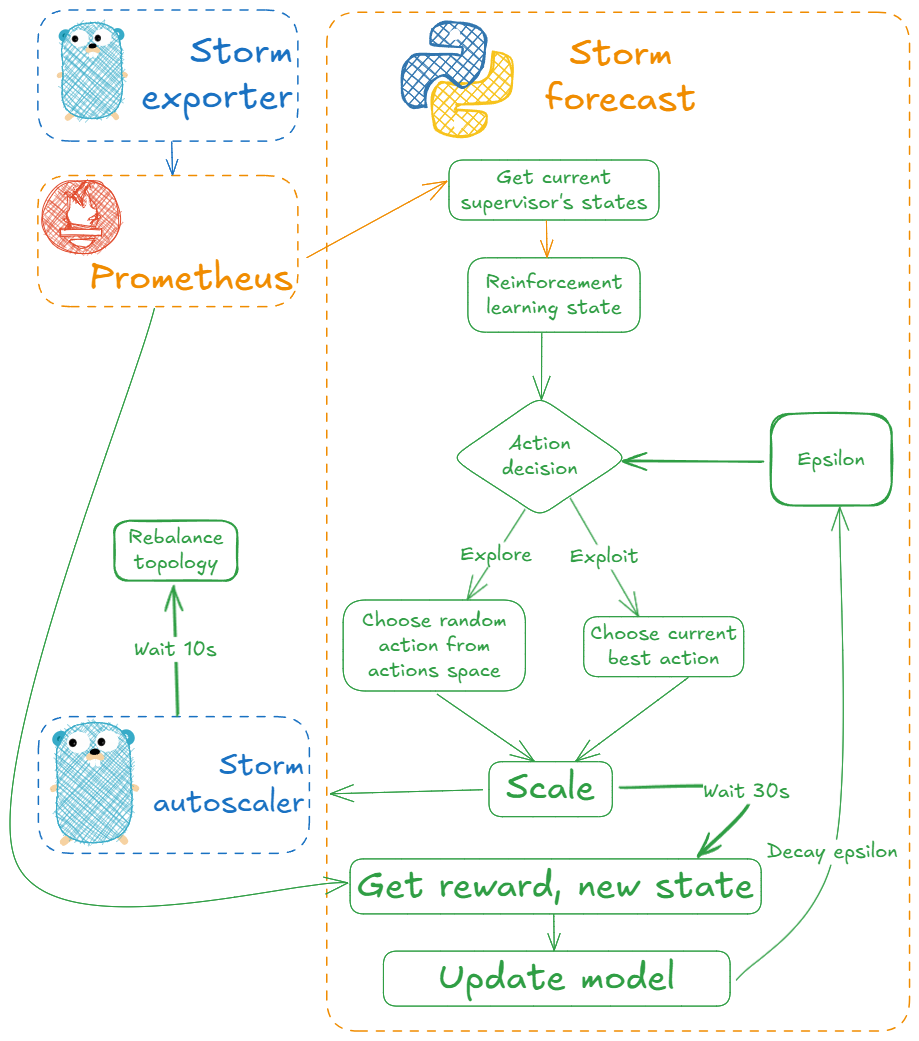
\includegraphics[width=\textwidth]{forecast-workflow.png}
    \caption{Sơ đồ luồng dự đoán tài nguyên}
\end{figure}

Hệ thống giám sát sử dụng Prometheus để thu thập và lưu trữ dữ liệu chỉ số được cung cấp từ Storm Exporter. Thành phần Storm Forecast sẽ khai thác các dữ liệu này nhằm dự đoán xu hướng sử dụng tài nguyên của các Supervisor trong tương lai, từ đó đưa ra quyết định co/dãn phù hợp và đánh giá hiệu quả hành động của mình. Toàn bộ quy trình hoạt động được mô tả theo các bước như sau:

\begin{itemize}
    \item Storm Forecast truy xuất các chỉ số hoạt động của Supervisor từ Prometheus. Các chỉ số thu được sẽ trải qua quá trình xử lý nhằm chuyển đổi thành biểu diễn trạng thái của môi trường học tăng cường, làm cơ sở cho việc ra quyết định.
    \item Dựa trên trạng thái hiện tại, tác nhân học tăng cường trong Storm Forecast sẽ chọn lựa hành động theo chính sách cân bằng giữa khám phá (exploration) và khai thác (exploitation). Sau khi hành động được xác định, hệ thống chuyển tiếp lệnh đến Storm Autoscaler để thực hiện. Storm Autoscaler sau khi tiến hành co/dãn số lượng supervisor và đợi 10 giây sẽ yêu cầu Storm Nimbus tái cân bằng lại topology để phân bổ lại các tiến trình worker vào các supervisor mới.
    \item Sau khi hành động được áp dụng, các chỉ số hệ thống tiếp tục được cập nhật thông qua Prometheus. Những dữ liệu mới này sẽ được phân tích để xác định phần thưởng nhận được, đồng thời thiết lập trạng thái tiếp theo của môi trường. Các thông tin này giúp điều chỉnh và cập nhật mô hình huấn luyện, tăng cường tri thức, từ đó cải thiện chất lượng quyết định trong tương lai.
    \item Cập nhật giá trị $\varepsilon$ để giảm xác suất khám phá khi hiểu biết về môi trường của tác nhân tăng lên theo thời gian.
    \item Chu trình huấn luyện được lặp lại liên tục vô hạn lần các chương, mỗi chương gồm nhiều lần hành động và kết thúc khi đạt tới số vòng lặp hoặc điều kiện dừng đã định trước. Mô hình được liên tục cập nhật và lưu vào ổ đĩa. Khi kết thúc giai đoạn huấn luyện, mô hình sẽ được sử dụng để phục vụ cho các giai đoạn đánh giá tiếp theo.
    \item Trong giai đoạn đánh giá, hệ thống sử dụng mô hình đã học được để đưa ra quyết định, điều này giúp giảm thiểu chi phí thiệt hại so với việc để tác nhân học từ đầu trên môi trường thực. Để đảm bảo khả năng thích nghi với biến động của môi trường, việc cập nhật mô hình vẫn được tiếp tục diễn ra.
\end{itemize}

\subsection{Đầu vào của Storm Forecast}

Mỗi trạng thái trong môi trường được biểu thị bởi bốn tham số:

\begin{enumerate}
    \item Trung bình tỷ lệ sử dụng bộ nhớ của toàn bộ các supervisor.
    \item Tổng số lượng gói tin các spout gửi đi.
    \item Tổng số lượng gói tin các spout gửi đi tại trạng thái trước đó.
    \item Số lượng supervisor hiện tại.
\end{enumerate}

Ngoài ra, tham số tỷ lệ sử dụng CPU đã từng được cân nhắc, nhưng sau đó bị loại bỏ do Docker sử dụng công thức tính CPU khác biệt, có thể dẫn đến giá trị vượt quá 100\% và sai khác giữa các môi trường là rất lớn (hình \ref{fig:gcp-cpu-usage} và hình \ref{fig:compose-cpu-usage}). Chính vì vậy, tham số này không đảm bảo tính ổn định khi áp dụng giữa môi trường huấn luyện (máy chủ nội bộ) và môi trường đánh giá (máy ảo trên nền tảng điện toán đám mây).

\begin{figure}
    \centering
    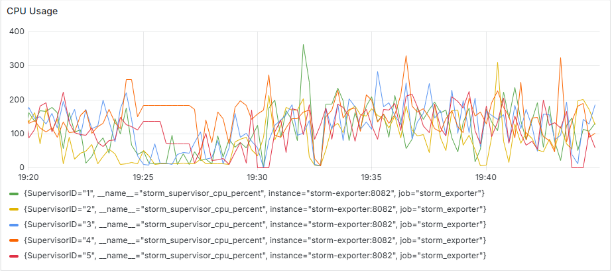
\includegraphics[width=\textwidth]{training-cpu-usage.png}
    \caption{Tỷ lệ sử dụng CPU của các supervisor trong môi trường điện toán đám GCP}
    \label{fig:gcp-cpu-usage}
\end{figure}

\begin{figure}
    \centering
    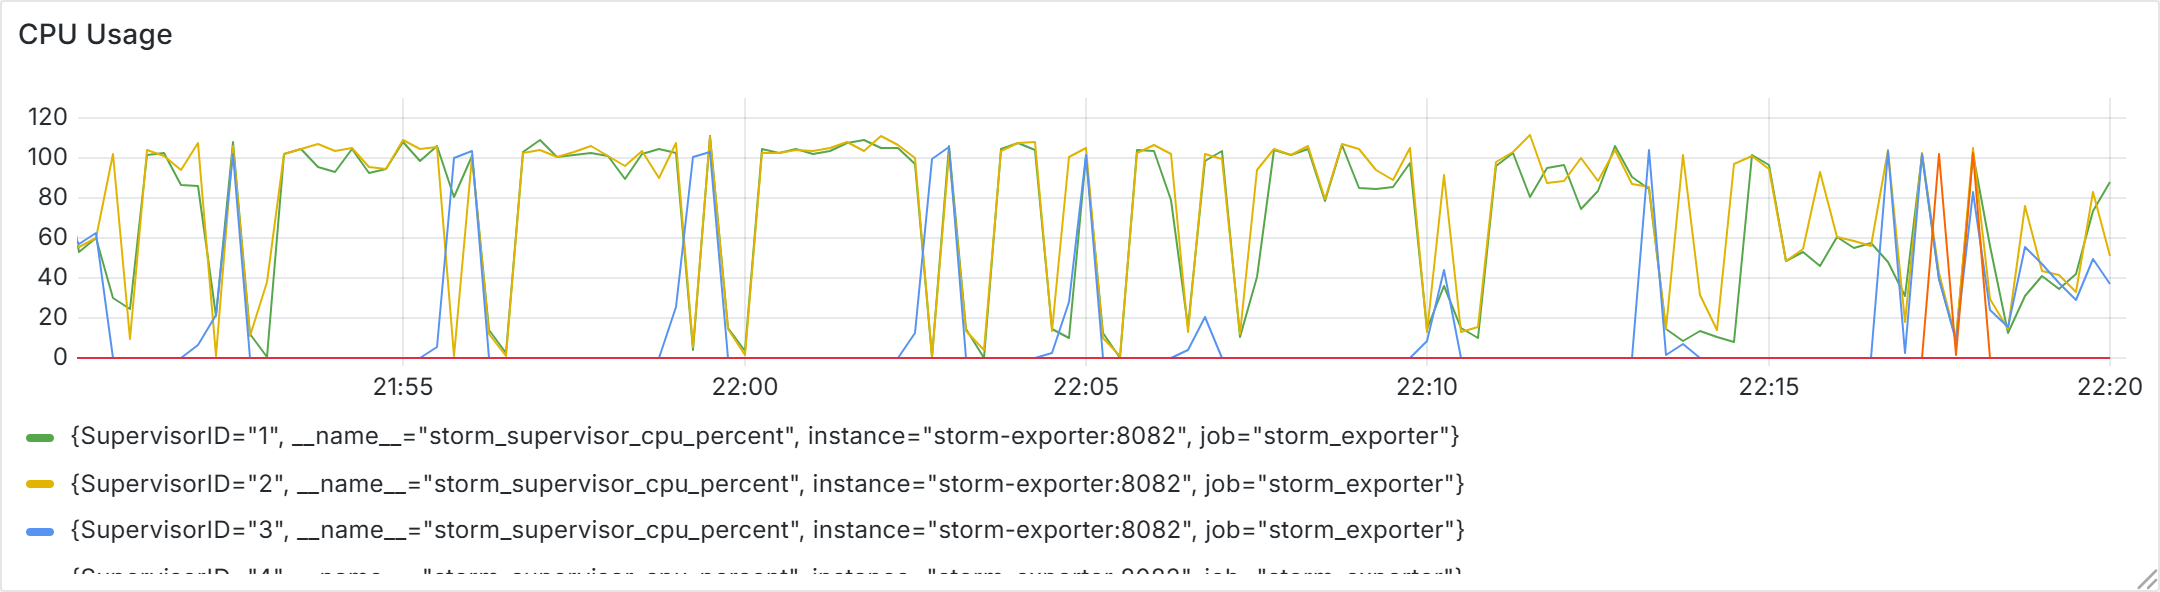
\includegraphics[width=\textwidth]{grafana-cpu-usage.png}
    \caption{Tỷ lệ sử dụng CPU của các supervisor trong môi trường Docker Compose}
    \label{fig:compose-cpu-usage}
\end{figure}

Các tham số được truy vấn và tính trung bình trong khoảng thời gian 20 giây gần nhất để tránh các trường hợp tham số có giá trị cao hoặc thấp đột biến gây sai lệch trong việc đánh giá.

\paragraph{Đầu vào của thuật toán Q-learning}
Trong Q-learning, trạng thái và hành động đều cần ở dạng rời rạc để làm chỉ số cho bảng Q. Khi trạng thái có dạng liên tục, không thể lưu trữ đầy đủ mọi giá trị vào bảng, dẫn đến không thể tra cứu hoặc cập nhật chính xác. Để giải quyết vấn đề này, tác giả áp dụng kỹ thuật thường được sử dụng gọi là state discretization (tạm dịch: phân rời hóa trạng thái), quá trình biến đổi được minh họa tại hình \ref{fig:flows-state-discretization}.

\begin{figure}[H]
    \centering
    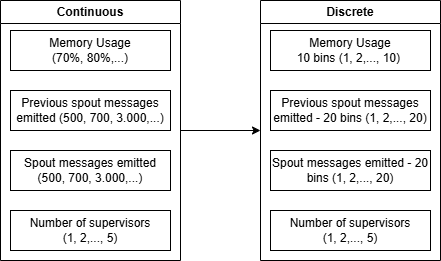
\includegraphics{flows-state-discretization.drawio.png}
    \caption{Sơ đồ minh họa phân rời hóa trạng thái}
    \label{fig:flows-state-discretization}
\end{figure}

\paragraph{Đầu vào của thuật toán học Q sâu}

Trong các mô hình học tăng cường sâu, đặc biệt là học Q sâu (Deep Q-Learning), việc chuẩn hóa đầu vào đóng vai trò quan trọng trong việc đảm bảo hiệu quả và độ ổn định của quá trình huấn luyện. Cụ thể, dữ liệu đầu vào (trạng thái môi trường) thường có sự chênh lệch lớn về đơn vị đo lường, phạm vi và phân phối. Nếu không được chuẩn hóa, những đặc tính này có thể gây khó khăn cho mạng nơ-ron trong việc học các biểu diễn có ý nghĩa, dẫn đến hội tụ chậm hoặc không ổn định.

Chuẩn hóa giúp đưa các đặc trưng đầu vào về cùng một thang đo, thường là trung bình bằng 0 và độ lệch chuẩn bằng 1. Điều này giúp mạng học hiệu quả hơn bằng cách:

\begin{itemize}
    \item Tăng tốc độ hội tụ do gradient lan truyền ổn định hơn.
    \item Giảm nguy cơ bị mắc kẹt ở cực trị không mong muốn trong không gian hàm mất mát.
    \item Giúp các trọng số ban đầu của mạng hoạt động hiệu quả hơn khi mọi đặc trưng đều quan trọng như nhau.
\end{itemize}

Trong thiết kế hệ thống co/dãn, các trạng thái của hệ thống được chuẩn hóa như sau:
\begin{itemize}
    \item Tỷ lệ sử dụng bộ nhớ trung bình / 100.
    \item Trung bình số lượng gói tin gửi bởi các spout (trong trạng thái hiện tại và trước đó) / 100.000.
    \item Số lượng supervisor / Số lượng supervisor tối đa có thể.
\end{itemize}

\subsection{Hàm đánh giá phần thưởng}

Giá trị phần thưởng của mỗi hành động được đánh giá bởi bốn tham số thu được trong trạng thái kế tiếp.

\paragraph{Trung bình tỷ lệ sử dụng bộ nhớ}

Một yếu tố quan trọng đầu tiên cần được xem xét là trung bình tỷ lệ sử dụng bộ nhớ của toàn bộ các supervisor trong khoảng thời gian 20 giây gần nhất. Mức phạt liên quan đến yếu tố này được đánh giá dựa trên hai kịch bản cụ thể.

Thứ nhất, nếu số lượng supervisor đã đạt đến mức tối thiểu và tỷ lệ sử dụng bộ nhớ trung bình của tất cả các supervisor vẫn thấp hơn ngưỡng mục tiêu đã định (trong nghiên cứu này là 60\%), thì mức phạt sẽ được gán là 0. Điều này là do đây được xác định là một hành động tối ưu, khi hệ thống đang hoạt động với số lượng tài nguyên ít nhất có thể mà vẫn đảm bảo hiệu suất dưới mức tải cho phép.

Thứ hai, trong tất cả các trường hợp còn lại, hình phạt được tính dựa trên độ lệch giữa tỷ lệ sử dụng bộ nhớ thực tế và tỷ lệ mục tiêu (60\%), kết hợp với một hình phạt nặng nếu tỷ lệ sử dụng vượt quá các ngưỡng giới hạn, cụ thể là vượt quá 80\% hoặc thấp hơn 20\%.

\begin{equation}
    \begin{aligned}
        P_{\text{memory}}(s_t) & =
        \begin{cases}
            0,       & \text{nếu}\quad N_t = N_{\min} \quad \\[8pt]
                     & \text{và} \quad \bar{s}_t < M^*,     \\[8pt]
            -\left(
            \frac{
                \sqrt{\frac{1}{N_t} \sum\limits_{i=1}^{N_t} (s_{t,i} - M^*)^2}
            }{40}
            +
            \sum\limits_{i=1}^{N_t} \mathbb{I}\{s_{t,i} > 80 \ \vee\ s_{t,i} < 20\}
            \right), & \text{khác.}
        \end{cases}
    \end{aligned}
\end{equation}
trong đó,
\begin{itemize}
    \item $s_t = (s_{t,1},\dots,s_{t,N_t})$ là vector phần trăm bộ nhớ của từng supervisor tại thời điểm $t$.
    \item $N_t = |s_t|$: số supervisor tại thời điểm t.
    \item $N_{min}$, $N_{max}$: số lượng supervisor tối thiểu và tối đa có thể của hệ thống.
    \item $\bar s_t = \tfrac{1}{N_t}\sum_{i=1}^{N_t}s_{t,i}$: trung bình tỷ lệ sử dụng bộ nhớ.
    \item $M^*$: tỷ lệ sử dụng bộ nhớ lý tưởng (60\%).
    \item $\mathbb{I}$: hàm chỉ báo, có giá trị bằng 1 nếu điều kiện trong ngoặc xảy ra và bằng 0 trong các trường hợp khác.
\end{itemize}

Thành phần đầu tiên được chuẩn hóa bằng cách chia cho 40, tương ứng với khoảng cách lớn nhất từ tỷ lệ mục tiêu 60\% đến ngưỡng thấp nhất là 20\%.

\paragraph{Hình phạt chi phí vận hành}

Bên cạnh việc tối ưu hóa việc sử dụng bộ nhớ, tác nhân còn phải đối mặt với hình phạt chi phí vận hành. Nguyên tắc cơ bản của hình phạt này là số lượng supervisor càng lớn thì chi phí vận hành càng cao, và do đó, hình phạt càng lớn. Điều này khuyến khích tác nhân ưu tiên sử dụng ít tài nguyên hơn khi có thể, nhằm giảm thiểu chi phí liên quan đến việc duy trì và quản lý một số lượng lớn các supervisor. Hình phạt này là một hàm tuyến tính dựa vào số lượng supervisor hiện tại so với số lượng supervisor tối đa được quy định. Mục tiêu là tạo ra sự cân bằng giữa việc đảm bảo hiệu suất hệ thống (thông qua việc sử dụng đủ supervisor khi cần) và việc tối thiểu hóa chi phí vận hành (bằng cách giảm số lượng supervisor khi có thể mà không ảnh hưởng đến hiệu suất).
\begin{equation}
    P_{\text{cost}}(N_t) = \quad -\frac{N_t}{N_{\max}}
\end{equation}
trong đó,
\begin{itemize}
    \item $N_t = |s_t|$: số supervisor tại thời điểm t.
    \item $N_{min}$, $N_{max}$: số lượng supervisor tối thiểu và tối đa có thể của hệ thống.
\end{itemize}

\paragraph{Hình phạt độ trễ}

\begin{figure}
    \centering
    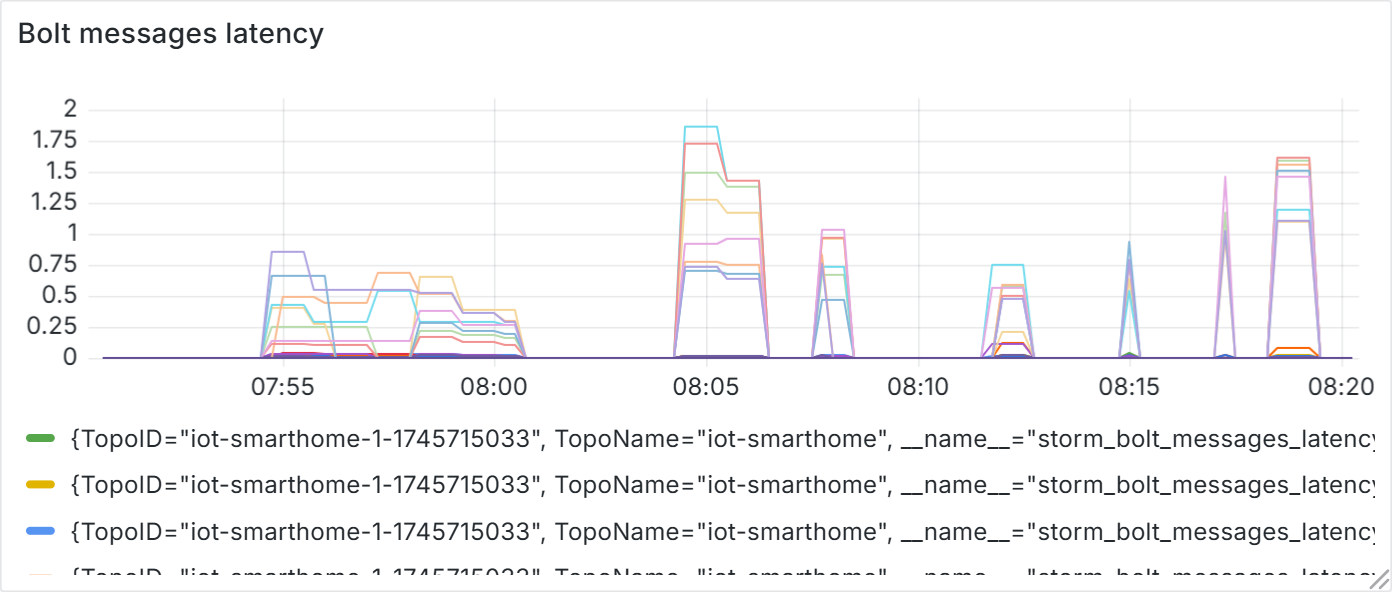
\includegraphics[width=\textwidth]{training-bolt-messages-latency.png}
    \caption{Độ trễ (ms) của các bolt trong quá trình huấn luyện}
    \label{fig:training-bolt-latency}
\end{figure}

\begin{figure}
    \centering
    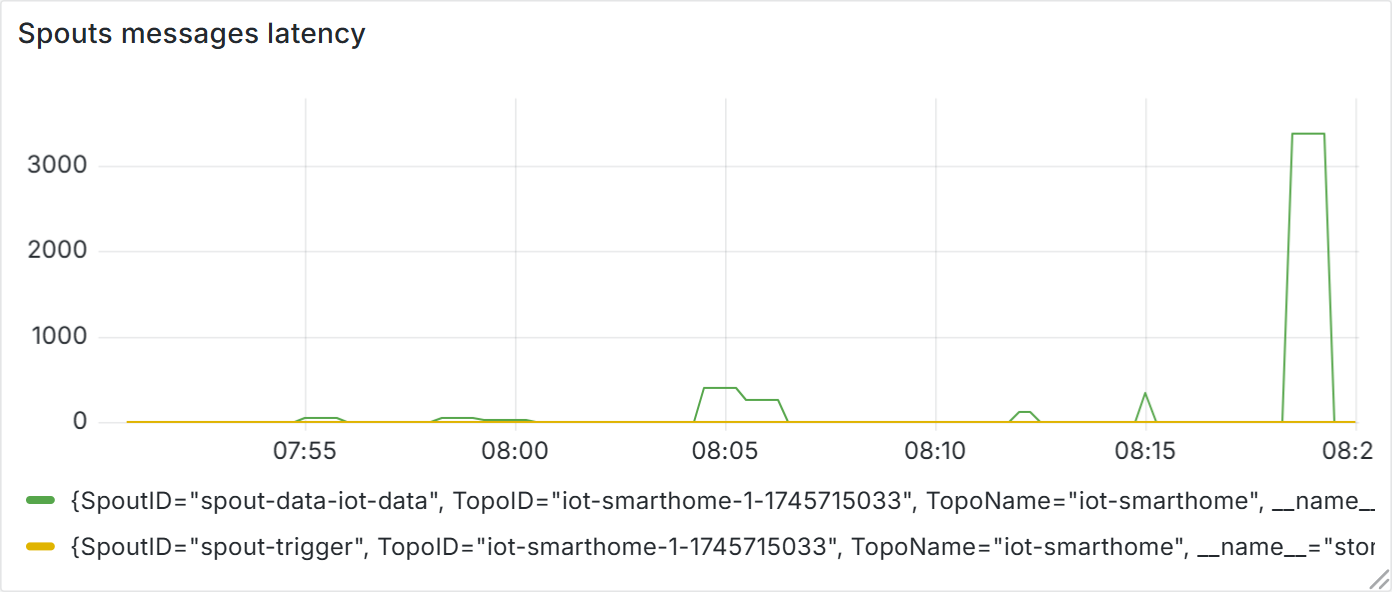
\includegraphics[width=\textwidth]{training-spout-messages-latency.png}
    \caption{Độ trễ (ms) của các spout trong quá trình huấn luyện}
    \label{fig:training-spout-latency}
\end{figure}
% \begin{figure}
%     \begin{minipage}{0.48 \textwidth}
%         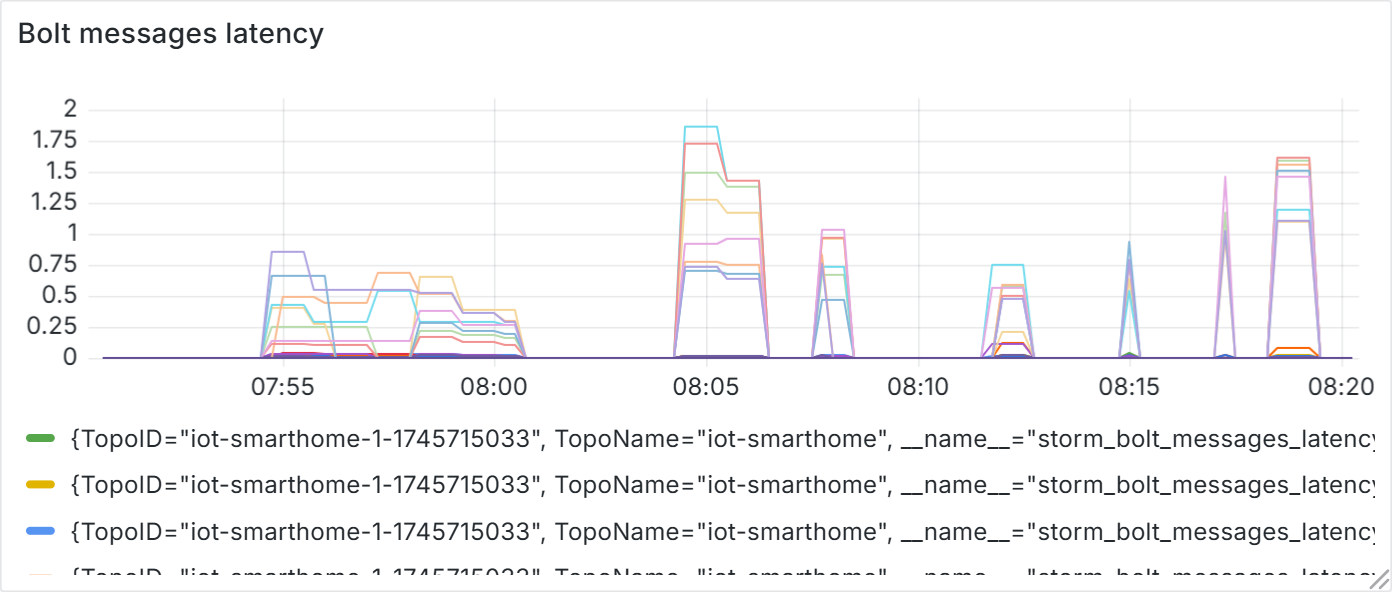
\includegraphics[width=\textwidth]{training-bolt-messages-latency.png}
%         \caption{Độ trễ của các bolt trong quá trình huấn luyện}
%         \label{fig:training-bolt-latency}
%     \end{minipage}
%     \begin{minipage}{0.48 \textwidth}
%         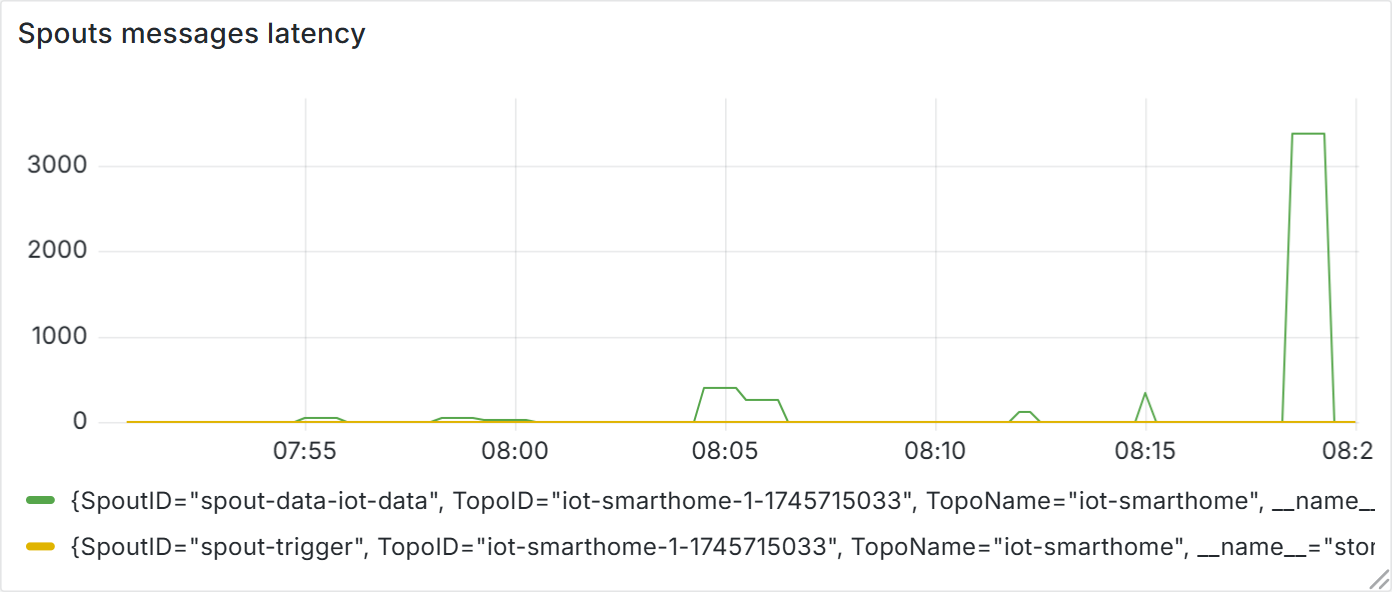
\includegraphics[width=\textwidth]{training-spout-messages-latency.png}
%         \caption{Độ trễ của các spout trong quá trình huấn luyện}
%         \label{fig:training-spout-latency}
%     \end{minipage}
% \end{figure}

Trong quá trình huấn luyện, dựa trên chỉ số thu thập được về độ trễ của các bolt hình \ref{fig:training-bolt-latency} và độ trễ của các spout hình \ref{fig:training-spout-latency}, có thể nhận thấy độ trễ của các spout thường lớn hơn đáng kể so với các bolt. Do spout đóng vai trò là nguồn đầu vào dữ liệu cho toàn bộ luồng xử lý, độ trễ cao ở thành phần này sẽ ảnh hưởng tiêu cực đến hiệu suất chung của hệ thống. Do đó việc đánh hình phạt cho độ trễ cũng đã được cân nhắc để có thể đảm bảo hệ thống hoạt động với hiệu suất cao, hiệu năng ổn định. Hình phạt này là một hàm tuyến tính dựa trên độ trễ hiện tại của tổng các gói tin của spout.

\begin{equation}
    P_{\text{latency}}(L_t) = -\,\frac{L_t}{1000}.
\end{equation}
trong đó,
\begin{itemize}
    \item $L_t$ là tổng độ trễ các gói spout tại thời điểm $t$.
\end{itemize}

\paragraph{Thưởng ổn định}

Tác nhân được nhận một phần thưởng nhỏ khi thực hiện hành động không thay đổi số lượng supervisor. Cơ chế này khuyến khích tác nhân duy trì trạng thái hiện tại, hướng đến sự ổn định của cấu trúc topology Storm và giảm thiểu nguy cơ downtime phát sinh do các thay đổi supervisor không cần thiết. Ví dụ, trong tình huống hệ thống đang vận hành với 3 supervisor và tỷ lệ sử dụng bộ nhớ trung bình là 50\%, thay vì thực hiện hành động giảm bớt 1 supervisor (có thể dẫn đến việc 2 supervisor còn lại chịu tải tăng lên đến 75\%), phần thưởng ổn định sẽ tạo động lực để tác nhân ưu tiên giữ nguyên số lượng supervisor hiện có.

\begin{equation}
    R_{\text{stability}}(a_{t-1}) =
    \begin{cases}
        \quad 1, & \quad \text{nếu} \quad a_{t-1} = \text{không co dãn}, \\
        \quad 0, & \quad \text{khác}.
    \end{cases}
\end{equation}

trong đó, $a_{t-1}$ là hành động được thực hiện tại thời điểm $t-1$, tức là hành động mà tác nhân đã thực hiện trước khi đạt đến trạng thái hiện tại.

\paragraph{Phương trình hàm phần thưởng/hình phạt}

Dựa trên bốn tham số đã được liệt kê bên trên, tác giả đã xây dựng hàm phần thưởng/hình phạt $V(a, s')$ cho trạng thái kế tiếp $s'$ có dạng tổng quát như sau:
\begin{equation}
    \begin{split}
        V(a, s') = - \omega_{memory} \cdot P_{memory}(s'_{memory}) - \omega_{cost} \cdot P_{cost}(s'_{supervisor}) \\
        - \omega_{latency} \cdot P_{latency}(s'_{latency}) + \omega_{stable} \cdot R_{stable}(a)
    \end{split}
\end{equation}
trong đó:

\begin{itemize}
    \item $\omega_{memory}$, $\omega_{cost}$, $\omega_{latency}$, $\omega_{stable}$ là các trọng số không âm, thể hiện tầm quan trọng tương đối của từng thành phần trong việc đánh giá.
    \item $R_{stable}(a)$, $P_{memory}(s'_{memory})$, $P_{cost}(s'_{supervisor})$, $P_{latency}(s'_{latency})$ được định nghĩa tương tự như trước.
    \item Dấu (-) trước các hành động thể hiện hình phạt thay vì dùng các trọng số âm sẽ gây phức tạp và dễ nhầm lẫn trong việc điều chỉnh các trọng số.
\end{itemize}

\subsection{Phương án lựa chọn hành động}

Chiến lược lựa chọn hành động $\epsilon$-greedy được áp dụng như sau: tại mỗi bước ra quyết định, tác nhân sẽ tạo một số ngẫu nhiên $r \in [0, 1)$. Hành động được lựa chọn dựa trên sự so sánh giữa $r$ và giá trị $\epsilon$ hiện tại:
\begin{itemize}
    \item Nếu $r < \epsilon$, tác nhân thực hiện một hành động ngẫu nhiên từ tập các hành động khả thi.
    \item Nếu $r \geq \epsilon$, tác nhân lựa chọn hành động có giá trị ước tính cao nhất theo hàm giá trị hiện tại.
\end{itemize}

Trong giai đoạn huấn luyện, giá trị $\epsilon$ ban đầu được thiết lập là $1.0$ và giảm theo cấp số mũ được thiết lập tùy thuộc theo thuật toán sau mỗi bước cho đến khi đạt ngưỡng tối thiểu là $0.05$. Ngược lại, trong giai đoạn đánh giá, giá trị $\epsilon$ được khởi tạo ở mức $0.05$, tương ứng với giá trị tối thiểu trong quá trình huấn luyện. Giá trị $\epsilon$ này đảm bảo tỷ lệ khai phá (exploration) là $5\%$ trong mỗi lần lựa chọn hành động, tạo điều kiện cho tác nhân thích ứng với những thay đổi tiềm ẩn của môi trường.